\documentclass{beamer}
\usepackage{graphicx}
\usepackage{subcaption}
\newtheorem{proposition}{Proposition}
\title{On the Universally Good Activation Function for One Node Neural Network}
\author{Feng Zhao}
\begin{document}
\begin{frame}
	\titlepage
\end{frame}
\begin{frame}
\frametitle{Function Approximation Problem}
\begin{figure}
	\centering
	\begin{subfigure}{0.4\textwidth}
		\includegraphics[width=\textwidth]{f1.png}
		\caption{wiggly function $f(x)$ to be approximated}
	\end{subfigure}~~~~~
	\begin{subfigure}{0.4\textwidth}
		\includegraphics[width=\textwidth]{f2.png}
		\caption{there is a one-hidden layer neural network to approximate $f(x)$ well [1]}
	\end{subfigure}
\end{figure}
The activation function is vital to the expressive power of enural networks.
\vskip 0.7cm
{\tiny Gybenko, G. "Approximation by superposition of sigmoidal functions." Mathematics of Control, Signals and Systems 2.4 (1989):
303-314.}
\end{frame}
\begin{frame}
\frametitle{One Node Neural Network Model}
\begin{columns}
\column{5cm}
\begin{figure}
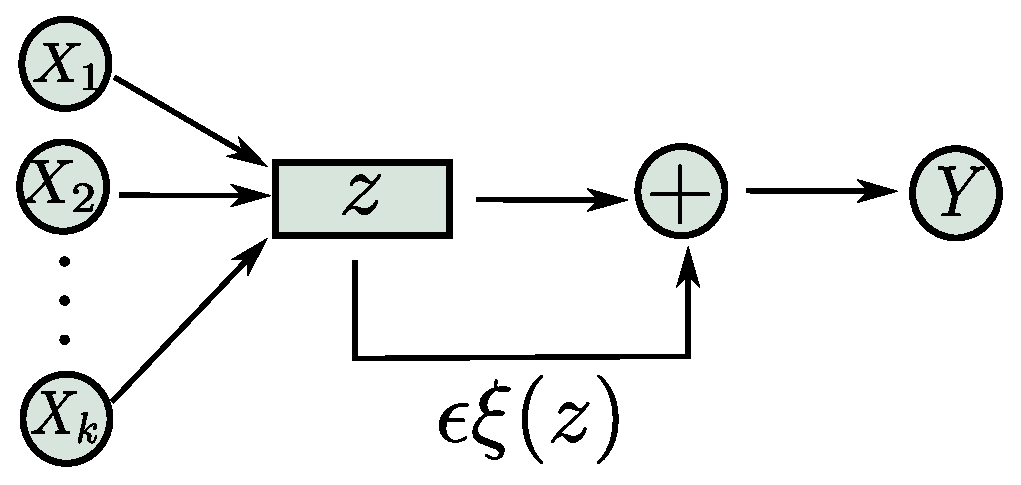
\includegraphics[width=\textwidth]{../network_structure.eps}
\end{figure}
\column{5cm}
Notations:
\begin{enumerate}
\item $X: n \times k$ random orthogonal matrix
\item $n :$ number of samples
\item $k: $ number of nodes in network 
\item $Y: n \times 1$ Gaussian vector
\end{enumerate}
\end{columns}
\vskip 0.5cm
Assume $X,Y$ are independent and $\epsilon$ is small, which $\sigma(z) = z + \epsilon \xi(z)$ can minimize the averaged estimation error $E(\sigma)$?
$$
E(\sigma)= \mathbb{E}[\min_{w} || Y - \sigma(X w) ||^2]
$$
\end{frame}
\begin{frame}
\frametitle{Our conclusions}
\begin{proposition}
Suppose $\xi(z)$ is a polynomial no more than $m$-order and $m\ll k$, then the optimal $\xi$ is $\xi_m(z) = \frac{1}{\sqrt{m! n}}H_m(\frac{n}{\sqrt{k}} z)$ and the optimal value is
$$
E(\sigma) = 1-\frac{k}{n}  - (1-\frac{k}{n})(m-1)  \epsilon^2 + o(\epsilon^2)
$$
\end{proposition}
\begin{block}{Further Discussion}
\begin{enumerate}
\item Non-linearity decreases the average approximation error
\item The decrasing rate is linear with polynomial order asymptotically
\end{enumerate}
\end{block}
\end{frame}
\end{document}